
\chapter{AI can be Jerks: Learning from the Best}

The previous story saw our protagonist start her carrer, and our
essays will begin with foundational material.  What a lay user needs
to understand what's happening in the story and how realistic it is.
We'll save the more fanciful and complicated stuff for later chapters.

For the moment, we focus on a facet of artificial intelligence called
machine learning.  Machine learning is a small subset of artificial
intelligence,\footnote{Research is organized around conferences; these
  onferences often form a community that is protective of its turf.
  While there is substantial overlap between the communities (e.g.,
  the Neural Information Processing Systems conference), many machine
  learning researchers (e.g., the International Conference on Machine
  Learning) prefer to remain distinct from ``pure'' artificial
  intelligence.} but unlike much of the fancifal claims of aritificial
intelligence prophets, it actually works \emph{now}.

We first introduce a key component of machine learning---objective
functions---that define why systems act they way they do. We then show
how bad human behavior can be mimicked by these algorithms (it's
already happening!).  Finally, we close the chapter with a call to
action: keep your computers safe!

\section{Learning by Doing: Objective Functions}
\label{sec:objective-functions}

Let us begin with an essential and underappreciated example of machine
learning that simply works and makes modern life liveable: spam
filters.  An e-mail is either spam or not; computers think in ones and
zeros, so let's call spam a one and not spam a zero.

An algorithm does not just say ``yes'' or ``no'' to whether an e-mail
is spam.  It typically gives a score for each e-mail: the higher the
score, the more confident it is the e-mail is spam.  For the moment,
let's assume that all of the numbers are between zero and one (e.g.,
they are a probability).

A perfect score would be if all spam e-mails got a 1.0 and all of the
good e-mails got 0.0.  Both perfection and absolute certainty are
unattainable goals, so we need to deal with both errors and
uncertainty.  So we sum all of the spam documents and see how far the
scores are from 1.0, and we sum all of the good e-mails and see how
far the scores are from 0.0.  This sum is our \emph{objective
  function}: a perfect score is 0.0 and the worst score is the number
of e-mails.

Machine learning algorithms are defined by \emph{parameters}.  For
example, a parameter might define what the algorithm does when it sees
the word ``viagra'' or the phrase ``I am a Nigerian prince''.  These
parameters effectively define the algorithm; machine learning
algorithms learn how to set these parameters from data, a process that
can take multiple names,\footnote{Some of the alternate names are
  field specific; for example, in statistics this is called inference
  and the objective function is typically called the likelihood.
  However, the mechanics are similar.  For some applications, it's
  called a ``loss function'', but we'll stick with the more general
  term.} but we'll call it ``optimization''.

\subsection{Optimization}

Optimization is the process where machine learning uses data to find
the parameters that give the best score on the objective function.
Typically, the process starts with a random setting of the parameters.
This will do \emph{horribly}, but it provides a place to start: the
early improvements will be easy.

The learning process will slowly change the parameters to ever so
slightly improve the objective function.\footnote{Mathematically, this
  is usually by looking at the gradient of the objective function with
  respect to the parameters.}  The learning process goes document by
document to slowly improve the objective function.  Eventually, modern
optimization techniques find a setting of the parameters that work
well for this problem.\footnote{The form of the objective function
  determines whether this answer will be the best possible or merely a
  ``good'' solution.}

All of this seems fairly straightforward, but there is some art to
creating these systems.  Defining the parameters requires a bit of
expertise: either hand-crafting parameters that fit the problem well
or using automatic approaches that learn effective representations.
Doing this well requires quite a bit of work, and often your first
(and second, etc.) attempt will usually fail.

\subsection{Is this Artificial Intelligence?}

A reasonable question is whether this is \emph{intelligence}.  Before
we get into the nuance of the question, the answer---given the systems
we have discussed---is definitely \textbf{no}.  But because we'll
discuss things that \emph{are} artificial intelligence later in the book, it's useful to
discuss what it means for a system to be intelligent now.  This way,
we can at least see why these systems are not intelligent.

In some ways, impressive achievements in technology is a moving
target.  After a few decades of living with machines that do a
formerly impressive task, we cease to be impressed by it and its
comparison to humans.\footnote{This is not just for intelligence;
  \song{The Ballad of John Henry} celebrates a competition between a
  steam drill and ``a man who ain't nothing but a man\dots with a
  hammer in [his] hand.''  Today, such comparisons and competitions
  seem silly.}  The luster of adding machines has faded into beige
quotidian boringness through the twentieth century.

Even in my own life, my excitement about halfway decent speech
recognition---taking a stream of speech and transcribing it into words
on a screen---has given way to annoyance at my phones' (increasingly
rare) mistakes.  Both of these were considered tasks that only humans
could do\footnote{The term ``computer'' originally referred to
  specially trained humans proficient at high-stakes, accurate
  calculations.} but now are so ubiquitous that half of humanity is
joined at the hip to devices that do both these things.

\TODO{Add cites}

However, these tasks can be framed as mechanical calculations; they
do not require abstract reasoning or generalization what people today
consider ``intelligence''.  More specifically, they requires hundreds
or thousands of examples to know what to do.  \energyJerk{} is a
prolific demonstrator of what (not) to do.  A human could learn
\energyJerk{}'s tricks from a high-level description.  An algorithm
learns to copy.  We discuss 

This simple mimicry can seem sophisticated.  It's couched in terms
that sound sophisticated but only facilitate superficial copying
(Figure~\ref{fig:la-ml}).  \energyCompany{} has a relatively simple
objective function to optimize: are people buying its
software or not?  If sales go up, it's good.  If sales go down, it's
bad.  Optimizing this function without any help is a difficult problem
(this is why \textsc{ceo}s are paid so much), but \energyCompany{}
doesn't have to do it alone: it learned it from \energyJerk{}.

\begin{marginfigure}%
  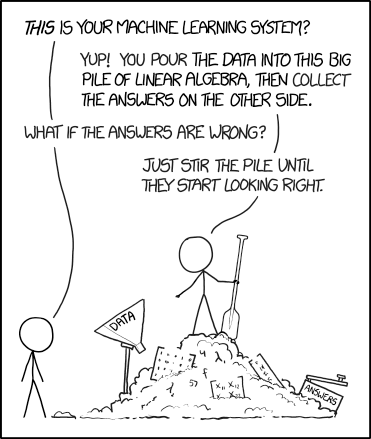
\includegraphics[width=\linewidth]{figures/xkcd-la-ml}
  \caption{Much of ``Machine Learning'' is copying in the form of
    complicated equations defined by mathematical formulas using fancy
    words like ``linear algebra'', ``gradients'', and ``nonconvex optimization''.}
  \label{fig:la-ml}
\end{marginfigure}

\subsection{Training Data}

We can now tie together the key concepts that we've introduced so
far.  \energyCompany{} 

\section{Humans are Jerks}

\quoted{Everybody's a jerk.  You, me, that jerk over there\dots
  That's my philosophy.}{Bender Bending Rodriguez, \series{Futurama}: \episode{I, Roomate}}

\subsection{I Learned it from You!}

\subsection{Prevention is Tough}

\section{Practicing Good Technology Hygene}

Stuxnet
